
\documentclass[../notes.tex]{subfiles}
\graphicspath{{\subfix{../img/}}}
\begin{document}

\part{ECE355: Signal Analysis and Communication}
\marginnote{Taught by Prof. Sunila Akbar}

\section{Admin and Preliminary}
\subsection{Lecture 1}
\begin{itemize}
	\item  CT and DT signals
	\item A ton of LTI (Linear time invariant) systems
	\item Processing of signals via LTI systems
	\item Fourier transforms
	\item Sampling
\end{itemize}
\subsubsection{Mark Breakdown}

\begin{table}[H]
	\centering
	\caption{Mark Breakdown}
	\begin{tabular}{|c|c|}
		\hline
		Homework & 20 \\
		MT1 & 20 \\
		MT2 & 20 \\
		Final & 40 \\
		\hline
	\end{tabular}
\end{table}

% \marginnote{HW is due two weeks after it is assigned}

\begin{itemize}
	\item Continuous enclose in (), independent is $ t $ 
	\item Discrete: enclose in [], independent is $ n $ 
\end{itemize}


\marginnote{In many systems we are interested in power and energy of signals over an infinite time interval; $ -\infty < \{ t, n \} < \infty$ }

\begin{theorem}
	\textbf{Energy for Complex Signals} 

	\begin{equation}
		E_{[t_1, t_2]} = \int_{t_1}^{t_2} \abs{x(t)}^2 dt
		\label{eq:355:energy_CT}
	\end{equation}

	\begin{equation}
		E_{[t_1, t_2]} = \sum_{n=n_1}^{n_2} \abs{x(t)}^2 dt
		\label{eq:355:energy_DT}
	\end{equation}

	\textbf{Average Power for Complex Signals} 

	\begin{equation}
		P_{avg, [t_1, t_2]} = \frac{1}{t_2 - t_1} \int_{t_1}^{t_2} \abs{x(t)}^2 dt
		\label{eq:355:power_avg_CT}
	\end{equation}

	\begin{equation}
		P_{avg, [t_1, t_2]} = \frac{1}{n_2 - n_1 + 1} \sum_{n=n_1}^{n_2} \abs{x(n)}^2
		\label{eq:355:power_avg_DT}
	\end{equation}
		
\end{theorem}


\section{Transformations}

\subsection{Lecture 2}
Most of this lecture was review. When applying transforms just note to always scale, \textit{then} shift, i.e.

\begin{enumerate}
	\item $ y(t) = x(\alpha t) $ 
	\item $ y(t) = x(\alpha t+\frac{\beta}{\alpha}) $ 
\end{enumerate}


\begin{definition}
	\textbf{Fundamental Period} 


	\begin{equation}
		x_t = x(t+ mT), m \in \mathbb{Z}
		\label{eq:355:fundamental_period}
	\end{equation}

	The fundamental period, $ T_o $  is the smallest positive value of $ T $ for which this holds true
\end{definition}

\begin{definition}
	\textbf{Even signals} 
	\begin{equation}
		x(t) = x(-t)
		\label{eq:355:even_signal}
	\end{equation}
\end{definition}

\begin{definition}
	\textbf{Odd signals} 
	\begin{equation}
		x(t) = -x(t)
		\label{eq:355:odd_signal}
	\end{equation}
\end{definition}


\begin{theorem}
	Any signal can be broken into an even and odd component

	\begin{equation}
		\begin{split}
			x(t) &= Ev \left\{ x(t) \right\} = \frac{1}{2} \left[ x(t) + x(-t) \right]  \\
			x(t) &= Od \left\{ x(t) \right\} = \frac{1}{2} \left[ x(t) + -x(-t) \right]  \\
		\end{split}
		\label{eq:355:even_odd_decomposition}
	\end{equation}
\end{theorem}


\subsection{Lecture 3}

Again, most of this lecture was review from the waves portion of PHY293 from last year or some other course prior.



A complex exponential and sinusoidal system can be represented as 
\begin{equation}
	x(t) = C e^{at}
\end{equation}

Where $ C, a $ are complex numbers.

Two cases may occur.

If $ a $ imaginary and $ C $ is real we have, depending on $ \omega $, either a constant signal or a periodic sinusoidal system.

\begin{equation}
	x(t_ = e^{j\omega_0t}) 
\end{equation}

\begin{itemize}
	\item Important property: this is periodic, i.e. $ Ce^{j\theta_0 t} = Ce^{j \theta (t + T)} $ 
	\item Implies that $ e^{j\omega_0T} = 1 $ 
	\item Implies that for $ \omega \neq  0 \rightarrow T_0 = \frac{2 \overline{n}}{|\omega_0|} $ 	
\end{itemize}


On the other hand, if $ a $ imaginary and  $ C $ complex, we have a periodic signal with $ T = \frac{2 \overline{n}}{\omega_0} $ 
\begin{equation}
	x(t) = Ce^{j\omega_0 t} = |C|e^{j\omega_0t + \phi} =  |C| \cos(\omega_o + \phi) + j|C| \sin(\omega_0 + \phi)
\end{equation}


The energy of the signal is given by \eqref{eq:355:energy_CT}, or


\marginnote{Recall: implication that $ e^{j\omega_0T} = 1 $, therefore the quantity inside the integral evaluates to $ 1 $  }

\begin{equation}
	E_{period} = \int^{T_0}_0 |e^{j\omega_0 t}|^2 dt = \int^{T_0}_0 1 dt = T_0
\end{equation}


\begin{equation}
	P_{period} = \frac{E_{period}}{T_0} = 1
\end{equation}



\subsubsection{General Continuous Complex Exponential Signals}


The most general case of a complex exponential can be represented as a combination of the real exponential and the periodic complex exponential;

\begin{equation}
		C = Ce^{at}
\end{equation}

and

\begin{equation}
	a = r + j\omega_0
\end{equation}

can be combined to give

\begin{definition}
	\begin{equation}
		Ce^{at} = |C|e^{rt}e^{j\omega_0t + \theta}
	\end{equation}
	Euler's relation can be used to simplify this to


	\begin{equation}
		Ce^{at} = |C|e^{rt} \left( \cos(\omega_0t + \theta) + j \sin(\omega_0t + \theta) \right)
	\end{equation}
\end{definition}


By inspection we can see that the signal has the following properties:

\begin{enumerate}
	\item $ r = 0 $: real and imaginary parts of sinusoidal
	\item $ r > 0 $: sinusoidal signal with exponential growth
	\item $ r < 0 $: sinusoidal signal with exponential decay
\end{enumerate}


I will be skipping notes on the discrete case as it is essentially the same as the continuous case, but with the following differences

\begin{table}[H]
	\centering
	\caption{Comparison of continuous and discrete complex exponential signals}
	\label{tab:label}
	\begin{tabular}{|p{0.4\linewidth}|p{0.4\linewidth}|}
		\hline
	 $ e^{j\omega_0t} $ & $ e^{j\omega_0n} $   \\ \hline
	 Distinct signals for distinct $\omega_{0} $ & identical signals for distinct $ \omega_0 \in \{\omega_0 \pm 2\pi i, i \in \mathbb{Z}\} $   \\ \hline
	 Periodic for any $ \omega_0 $ & Periodic only if $ \omega_0 = \frac{2\pi m}{N}  $ for integers $ N>0, m $  \\ \hline
	 Fundamental frequency  $ \omega_0 $ & Fundamental frequency $\frac{\omega_0}{m}$  \\ \hline
	 Fundamental period $ \omega_0 = 0 \rightarrow $ undefined, otherwise $ T_0 = \frac{2\pi}{\omega_0} $ & Fundamental period $ \omega_0 = 0 \rightarrow $ undefined, otherwise $ T_0 = m\frac{2\pi}{\omega_0} $  \\ \hline
																																																				& Since unique $ \omega $ does not mean unique signal, pick $ 0 \le \omega_0 \le 2\pi $ or $ -\pi \le \omega_0 \le  \pi$  \\
	 \hline
	\end{tabular}
\end{table}

\section{Basic Signals}

\subsection{Lecture 4: Step and Impulse Functions}

One of the simplest discrete-time signals is the \textbf{unit impulse}\sidenote{or unit sample} function, $ \delta[n] $ 


\begin{definition}
\begin{equation}
	\delta[n] = \begin{cases}
		0 & n \neq 0 \\
		1 & n = 0
	\end{cases}
	\label{eq:355:unit_impulse}
\end{equation}


\begin{figure}[H]
	\centering
	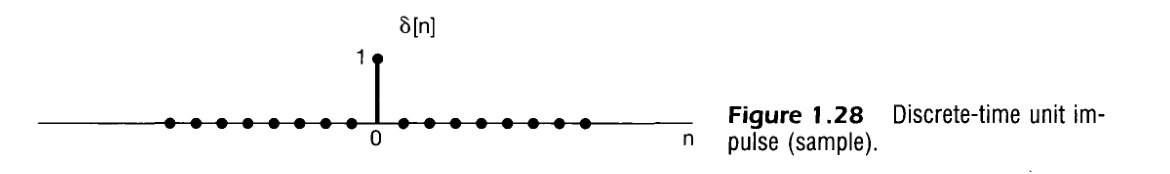
\includegraphics[width=0.8\linewidth]{img/image_2022-09-16-14-12-45.png}
\end{figure}
\end{definition}


Another basic signal is the \textbf{unit step} function, $ u[n] $

\begin{definition}
	
\begin{equation}
	u[n] = \begin{cases}
		0 & n < 0 \\
		1 & n \geq 0
	\end{cases}
\end{equation}
\begin{figure}[H]
	\centering
	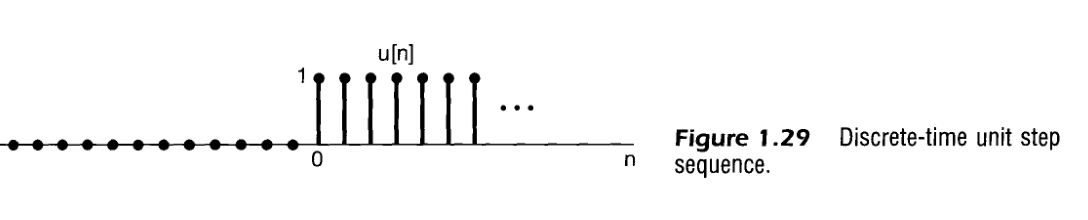
\includegraphics[width=0.8\linewidth]{img/image_2022-09-16-14-13-03.png}
\end{figure}
\end{definition}


The unit impulse function is the first difference of the discrete time step function, i.e.

\begin{equation}
	\delta[n] = u[n] - u[n-1]
\end{equation}

And the unit step function is the running sum of the unit impulse function, i.e.

\begin{equation}
	u[n] = \sum_{m=-\infty}^n \delta[m]
\end{equation}

This can be rewritten with $ k = n-m $ to make a more convenient expression for moving the function along $ -\infty\ldots0\ldots\infty $ 

\begin{equation}
	u[n] = \sum_{k=0}^\infty \delta[n-k]
\end{equation}




\begin{theorem}
	
The unit impulse function $ \delta[n-n_0] $ can be used to sample a function at a specific $ n = n_0 $ since the impulse function will take on the value $ 0 $ for all values of $ n \neq  n_0$ 
\begin{equation}
	x[n] \delta[n-n_0] = x[n_0]\delta[n-n_0]
\end{equation}
\end{theorem}





The continuous equivalents of the unit impulse and unit step functions are defined similarly

\begin{definition}
	
\begin{equation}
	u(t) = \begin{cases}
		0 & t < 0 \\
		1 & t > 0
	\end{cases}
\end{equation}
\end{definition}


Likewise, the continuous unit step function is a running \st{sum} integral of the continuous unit impulse function

\begin{equation}
	u(t) = \int^{t}_{-\infty} \delta(\tau)d\tau
	\label{eq:355:unit_step_cont}
\end{equation}


A relationship analogous to the discrete case can be found for the continuous case; the continuous unit impulse function can be thought of as the first derivative of the continuous-time unit step function

\begin{definition}
\begin{equation}
	\delta(t) = \frac{du(t)}{dt}
	\label{eq:355:unit_impulse_continuous}
\end{equation}
	
\end{definition}


\eqref{eq:355:unit_impulse_continuous} is discontinuous at $ t=0 $ so it is non-differentiable. We can address this by considering an approximation of \eqref{eq:355:unit_impulse_continuous} for a $ \Delta $ short enough to not matter for any practical purpose

\begin{figure}[H]
	\centering
	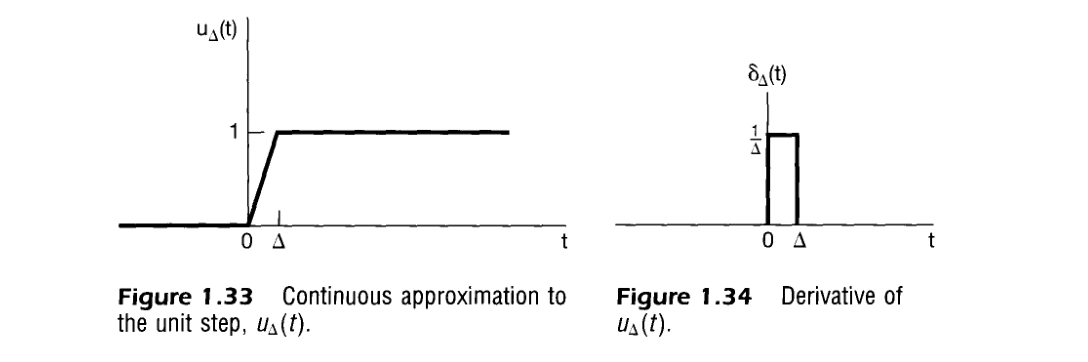
\includegraphics[width=0.8\linewidth]{img/image_2022-09-16-16-53-20.png}
\end{figure}


\eqref{eq:355:unit_step_cont} can be rewritten as follows to make it more convenient to use along $ \sigma\in-\infty\ldots 0\ldots\infty$. 

\begin{equation}
	u(t) = \int^{\infty}_0 \delta(t-\sigma) d\sigma
\end{equation}

\begin{theorem}
	
And by the same argument as for the discrete case, the continuous impulse function has an important sampling property.

	For any arbitrary point $ t_0 $,

	\begin{equation}
		x(t) \delta t(t-t_0) = x(t_0)\delta(t-t_0)
	\end{equation}

\end{theorem}

\subsection{Lecture 5}


\begin{definition}
	A \textbf{system} is a process that transforms a signal, i.e. 
	\begin{equation}
		x(t) \xrightarrow{\text{sys}} y(t)
	\end{equation}

	\marginnote{A similar definition can be applied for the discrete case}
	
\end{definition}


Some examples of the relationship between signals and physical systems include circuits, i.e. RLC circuits and spring-mass systems.

\begin{example}
	For example a RLC circuit can be modeled as a system that transforms a voltage signal into a current signal;
	\begin{figure}[H]
		\centering
		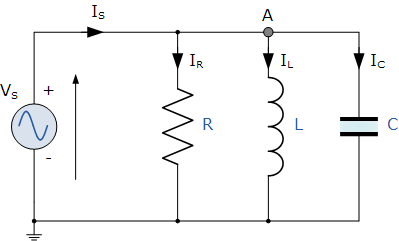
\includegraphics[width=0.8\linewidth]{img/image_2022-09-21-14-17-52.png}
	\end{figure}


	\begin{equation}
		v(t) \xrightarrow{\text{RLC}} i(t)
	\end{equation}

	Solving and modelling this system was covered in the other circuit classes.
\end{example}


Systems can be combined, i.e. making a mobile call

\begin{equation}
	a(t) \xrightarrow{mic} y(t) \xrightarrow{antenna} z(t) \xrightarrow{tower} u(t) \xrightarrow{antenna} w(t) \xrightarrow{speaker} b(t)
\end{equation}

\subsubsection{Types of systems}

\begin{figure}[H]
	\centering
	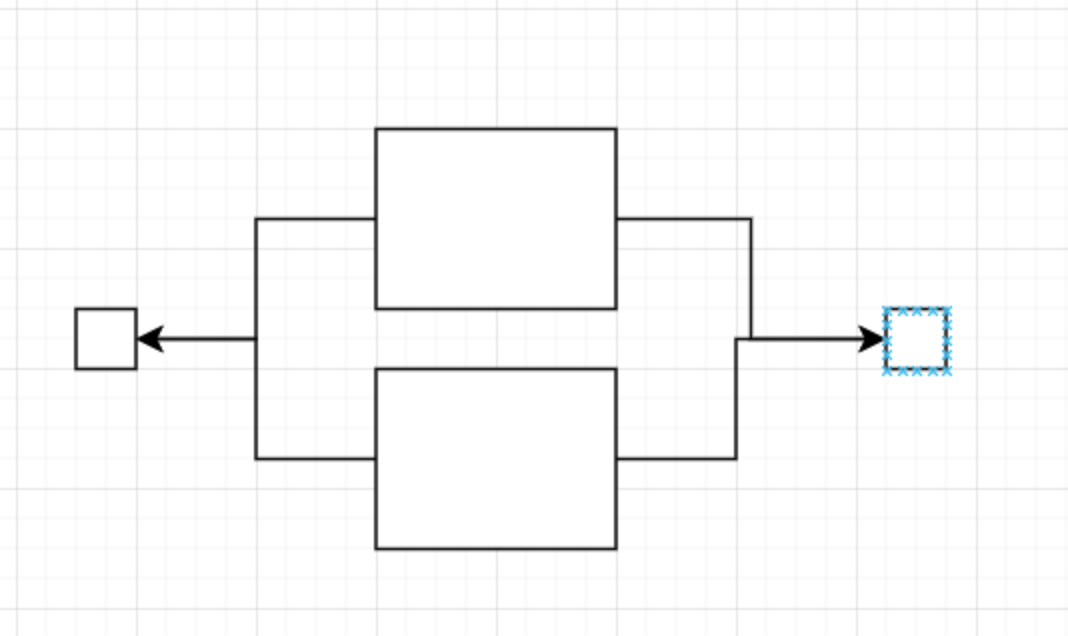
\includegraphics[width=0.8\linewidth]{img/image_2022-09-21-14-28-14.png}
	\caption{Parallel systems}
\end{figure}


\begin{figure}[H]
	\centering
	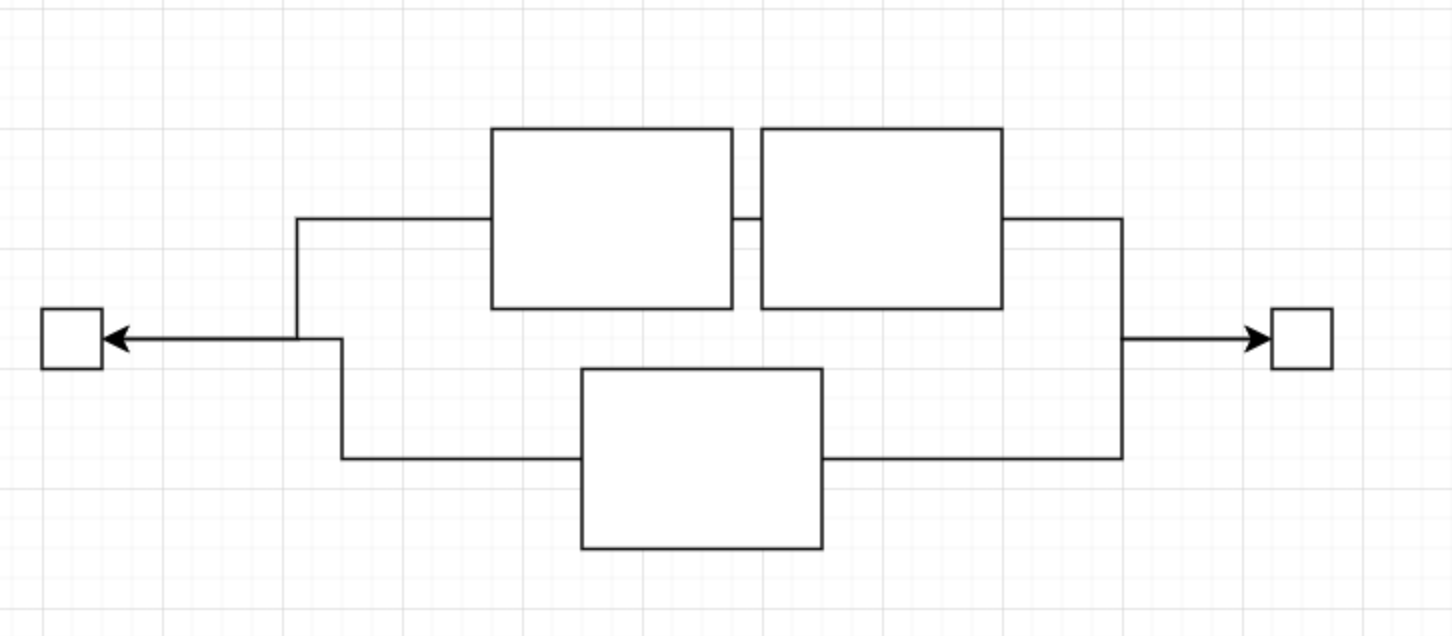
\includegraphics[width=0.8\linewidth]{img/image_2022-09-21-14-29-14.png}
	\caption{Series-parallel}
\end{figure}

\marginnote{The feedback control system will be discussed in depth in the control systems class}
\begin{figure}[H]
	\centering
	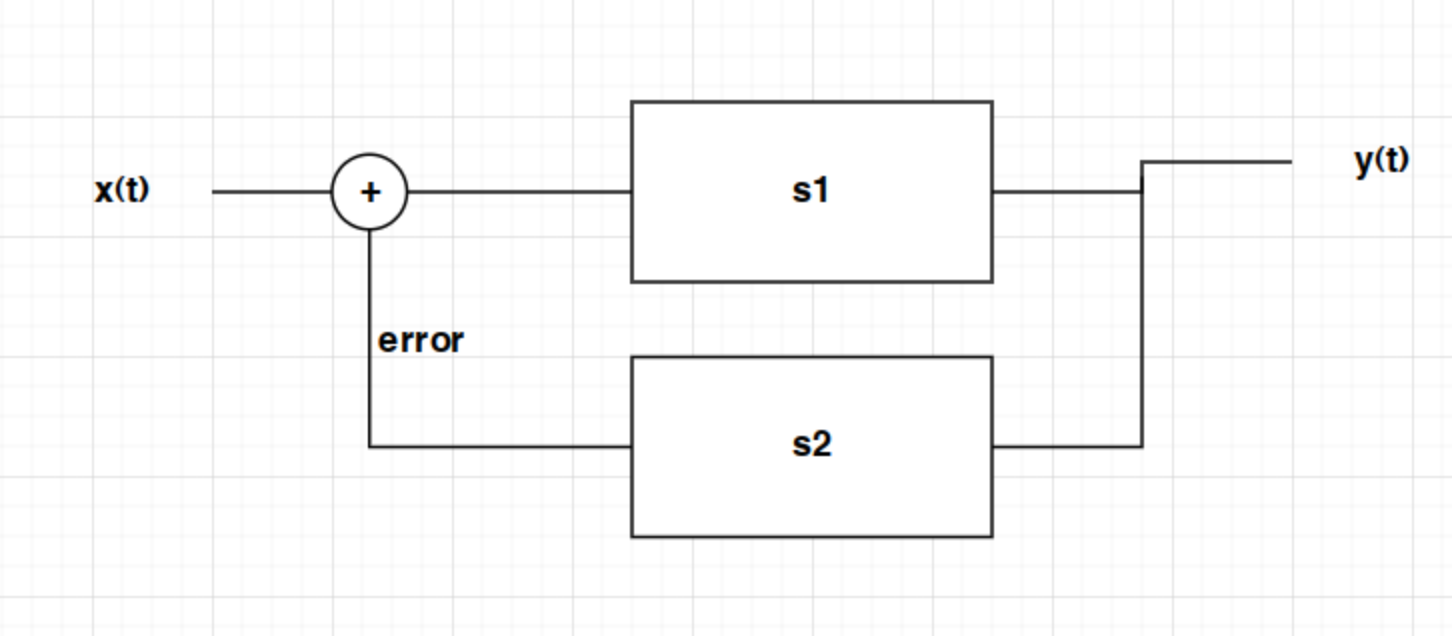
\includegraphics[width=0.8\linewidth]{img/image_2022-09-21-14-30-39.png}
	\caption{Feedback control system}
\end{figure}





\subsubsection{System properties}

\begin{definition}
	\textbf{Memoryless} systems are systems where its output of the independent variable at a given time is dependent only on  the input at the same time.

	For example,

	\begin{equation}
		y[n] = 2x[n] - x^2[n]
	\end{equation}
	is a memoryless system, but 
	\begin{equation}
		y[n] = 2x[n] - x^2[n-1]
	\end{equation}
	is not.
\end{definition}

Other simple memoryless systems include the identity system $ x(t) = y(t) $



A system with memory is the \textit{accumulator}  

\begin{equation}
	y[n] = \sum^n_{k=-\infty} x[k]
\end{equation}


A capacitor is an example of a continuous-time system with memory

\begin{equation}
	v(t) = \frac{1}{C} \int^{t}_{-\infty} i(\tau) d\tau
\end{equation}

There can also be systems that are dependent on future values of the input and output\mn{PID go brr}.



\begin{definition}
	A system is \textit{invertible} if distinct inputs lead to distinct outputs\mn{Recall: MAT185 and matrix investability}
	For example, the identity system is invertible, but the accumulator is not.
\end{definition}

\begin{definition}
	A system is \textit{casual} if its output at a given time is dependent only on the input at the current time and in the past.
\end{definition}

Then it follows that
\begin{lemma}
	All memoryless systems are casual
\end{lemma}

Though casual systems are useful, non-casual systems are also of great utility in modelling systems in which the independent variable is not time, or in \textit{anticipative} models that account for the future values of the input or output, i.e a controller.


\begin{definition}
	A system is \textit{stable} is if the output is bounded if the input is bounded.
\end{definition}


\begin{definition}
	A system is \textit{time invariant}  if the behaviour and characteristics are fixed over time.
	For example, a $ RC $ circuit is time-invariant if the circuit $ R, C $ values are constant over time. More formally, a system is time invarient if a time shift in the input signal results in an identical time shift in the output.

	If	
	\begin{equation}
		x[n] \xrightarrow{\text{sys}} y[n]
	\end{equation}

	Then, for a time invariant system,

	\begin{equation}
		y[n-n_0] \xrightarrow{\text{sys}} x[n-n_0]
	\end{equation}

\end{definition}

\begin{definition}
	A system is \textit{linear} if it possess the property of superposition, i.e. it possess the additive property and the scaling, or homogeneity property.

	More formally, a linear system is one such that

	\begin{equation}
		ax_1(t) + bx_2(t) \xrightarrow{\text{sys}} ay_1(t) + by_2(t)
	\end{equation}

	Where $ y_1 $ is the output of a system with input $ x_1 $ and $ y_2 $ is the output of a system with input $ x_2 $.
	
\end{definition}


\section{LTI systems}
\subsection{Lecture 6: Discrete LTI systems}
Many physical systems can be modelled as linear time-invariant (LTI) systems.
This is useful because there exists a large body of theory that can be applied to LTI systems, in part due to LTI systems possessing the superposition property.



\begin{figure}[H]
	\centering
	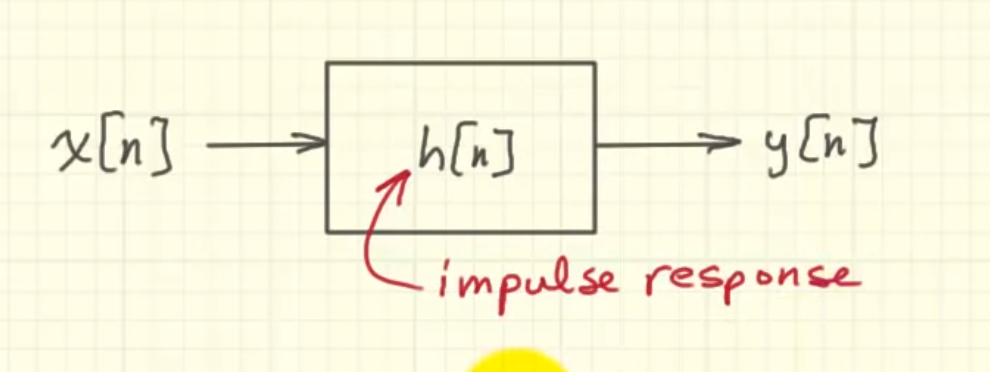
\includegraphics[width=0.8\linewidth]{img/image_2022-09-25-20-06-00.png}
	\caption{In this lecture the idea of LTI systems being a sum of $ h[n] $ impulse responses will be }
\end{figure}


\begin{theorem}
	Discrete signals can be represented as a summation of impulses.

	\begin{figure}[H]
		\centering
		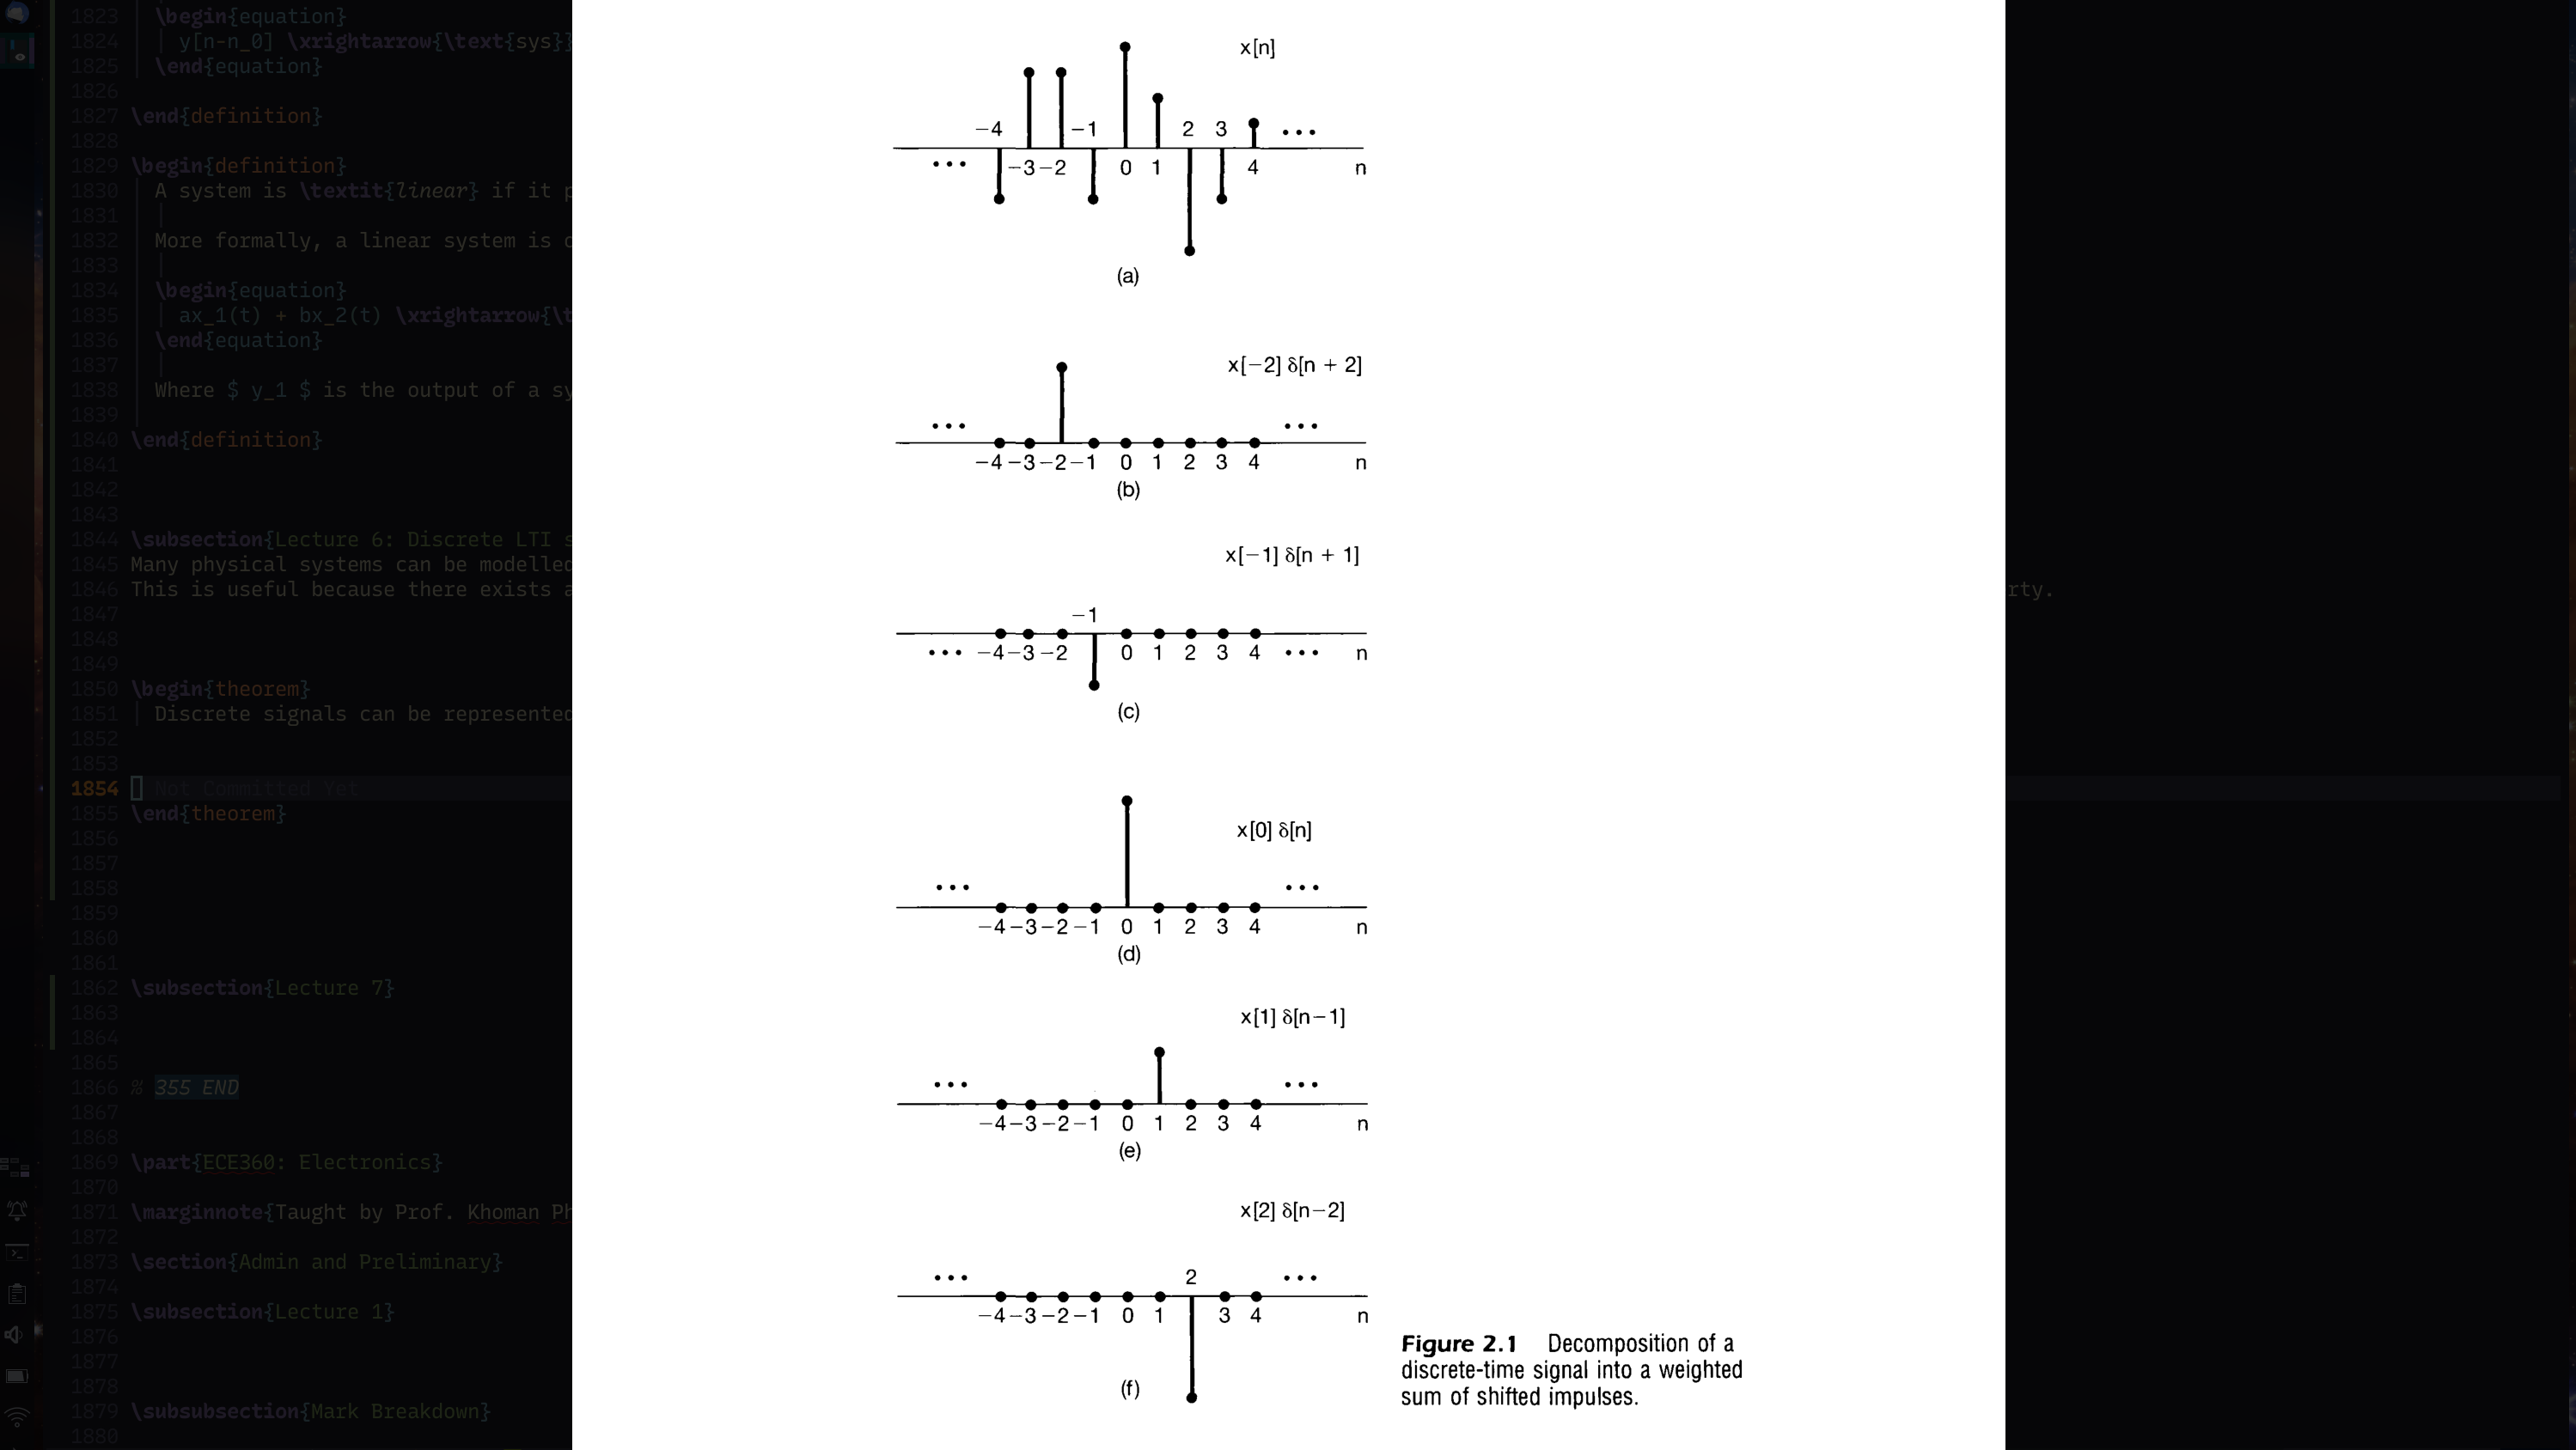
\includegraphics[width=\linewidth]{img/image_2022-09-22-13-51-38.png}
	\end{figure}

	More generally, a discrete signal can be rewritten as a sum of shifted unit impulses with weights $ x[k] $  

	\begin{equation}
		x[n] = \sum_{n=-\infty}^{\infty} x[k] \delta [n-k]
	\end{equation}

	\begin{example}
		As an example we can rewrite the unit step function as

		\begin{equation}
			u[n] = \sum_{n=0}^{\infty} \delta[n-k]
		\end{equation}
		\marginnote{
			The discrete unit impulse also possesses a \textit{sifting} property; since $ \delta[n-k] $  is nonzero only when $ k = n $, this summation will sift through the values of $ x[k] $ and preserves only the values corresponding to $ k = n $  
		}
		
	\end{example}

\end{theorem}

A useful result of the properties of LTI systems (i.e. the superposition property) is that the output of a system is the convolution of the input and the impulse response of the system, i.e.


\begin{definition}
	\textbf{Convolution} sum 
	
	\begin{equation}
		y[n] = \sum_{k=-\infty}^{\infty} x[k] h[n-k]
	\end{equation}
	\begin{theorem}

		An LTI system can be modelled as a \textbf{convolution} sum, or a sum of scaled and shifted impulse responses.
		So, if we know the response of the linear system to the set of shifted unit impulses -- we can determine the response of the system to any input signal!

\end{theorem}

Symbolically convolution can be written as
\begin{equation}
	y[n] = x[n] * h[n]
\end{equation}


\end{definition}





\subsection{Lecture 7: Continuous LTI systems}

The concept of a LTI system responding to unit impulses and taking advantage of the sifting property may be extended to the continuous systems by idealizing the pulse as one so short that it's duration is inconsequential for any real system.

\begin{definition}
	\textbf{Sifting property} of continuous-time impulse

	\begin{equation}
		x(t) = \int_{-\infty}^{\infty} x(\tau) \delta(t-\tau) d\tau
	\end{equation}

	Can interpret $ x(\tau)\delta(t-\tau) $ equals $ x(t) \delta(t-\tau) $, i.e. that it is a \textit{scaled impulse} 

	\begin{equation}
		x(t) = \int_{-\infty}^{\infty} x(\tau) \delta(t-\tau) d\tau = x(\tau) \int_{-\infty}^{\infty} \delta(t-\tau)  d\tau
	\end{equation}
	
	
\end{definition}

If we let $ h_\tau (t) $ denote the response at time $ t $ to an unit impulse $ \delta(t - \tau) $ at time $ \tau $, then


\begin{equation}
	y(t) = \lim_{\Delta \to 0} \sum_{k=-\infty}^{\infty} x(k\Delta) \hat{h}_{k\Delta} (t) \Delta
\end{equation}

As $ \Delta \to 0 $ the summation becomes an integral, i.e.

\begin{equation}
	y(t) = \int_{-\infty}^{\infty}   x(\tau) h_{\tau}  (t) d \tau
\end{equation}

For notational convenience the $ \tau $ subscript can be dropped and generalizing to all $ t $ 

\begin{equation}
	y(t) = \int_{-\infty}^{\infty}   x(\tau) h(t-\tau) d \tau
\end{equation}

Symbolically the convolution is represented $ y(t) = x(t) \cdot h(t)$ 


\subsection{Lecture 12}
A class of LTI systems that are really important are ones related through linear constant-coefficient differential equations.
For example, consider

\begin{equation}
	\frac{dy(t)}{dt} + 2 y(t) = x(t)
	\label{eq:355:l12_1}
\end{equation}

This equation offers an implicit specification of the system, i.e. a relationship between input and output instead of an explicit expression; to find a explicit expression we must plug in initial conditions.


Given the exponential input 

\begin{equation}
	x(t) = K e^{3t} u(T)
\end{equation}

to  \eqref{eq:355:l12_1}, the complete solution to a differential equation of this type is given as the sum of a particular and homogeneous solution\sn{Recall ESC195}

\begin{equation}
	y(t) = y_p(t) + y_h(t)
\end{equation}


A common method for finding the particular solution is to first look for the \textit{forced response}; an output signal with the same form as the input.

Take 

\begin{equation}
	y_p(t) = Ye^{3t}
\end{equation}

and then doing some math we find $ Y = \frac{K}{5} $ to arise at $ y_p(t) = \frac{K}{5}e^{3t}, t > 0 $.

To find the homogeneous solution we hypothesize a solution of form

\begin{equation}
	y_h(t) = Ae^{st}
\end{equation}

and then substitute into the differential equation to find

\begin{equation}
	y(t) = Ae^{-2t} + \frac{K}{5} e^{3t}, \qquad t > 0
\end{equation}

The constants $ A, K$ can then be found by substituting in the initial conditions.



More generally speaking, a $ N $th order linear constant-coefficient differential equation is given by

\begin{equation}
	\sum^N_{k=0} a_k \frac{d^k y(t)}{dt^k} = \sum^{M}_{k=0} b_k \frac{d^k x(t)}{dt^k}
\end{equation}


The discrete time counterpart is

\begin{equation}
	\sum_{k=0}^{N} a_k y[n-k] = \sum_{k=0}^{M} b_k x[n-k]
\end{equation}

With the solution $ y[n] $ being the sum of the particular solution to the problem above and a solution to the homogeneous equation

\begin{equation}
	\sum_{k=0}^{N} a_k y[n-k] = 0
\end{equation}



A important special case of LCCDEs are LTIs.

Consider a response to an arbitrary exponential input signal

\begin{figure}[H]
	\centering
	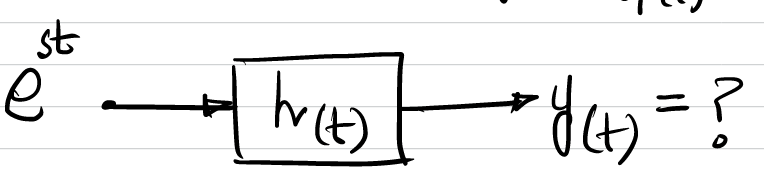
\includegraphics[width=0.8\linewidth]{img/image_2022-11-02-16-16-38.png}
\end{figure}


\begin{definition}
	\textbf{Laplace transform of $ h $}, or the transfer function of LTI systems
\begin{equation}
	y(t) = \int_{-\infty}^{\infty}  h(\tau) e^{-s\tau} d \tau = \int_{0}^{1}  e^{-s\tau}d\tau = \begin{cases}
		\frac{1}{s} (1-e^{-s}) & s \neq  0\\
		1 & s = 0
	\end{cases} 
\end{equation}



	
\end{definition}

\begin{theorem}
	If $ x(t) = e^{st} $ and $ H_s $ exists, $ y(t) = H(s) e^st $

	This can be interpreted in two ways

	\begin{enumerate}
		\item Same constant exponential as input	$e^{st} $ (eigenfunction of LTI system)
		\item Scaled by constant $ H(s) $ (eigenvalue)
	\end{enumerate}

	\textbf{Corollary} 

	If the input to an LTI system with an impulse response $ h(t) $ is 
	\begin{equation}
		x(t) = \sum_k a_k e ^{s_kt}
	\end{equation}
	
		then it's output is given by

		\begin{equation}
			y(t) = \sum_k a_k H_{s_k} e^{s_kt}
		\end{equation}
		

\end{theorem}

Since almost all periodic signals can be expressed as a sum of harmonically related complex exponentials, i.e.


\begin{equation}
	x(t) = 
	\sum_{k=-\infty}^{\infty} a_k e^{j k\omega_ t } = 
	\sum_{k=-\infty}^{\infty} a_k e^{j \frac{2\overline{n}k}{T}t}
\end{equation}

Where the $ k $ denotes the $ |k| $th harmonic component and $ a_0 $ being the constant component\sn{In circuit analysis this is the constant component}




\subsection{Lecture 15: Which periodic signals have a Fourier representation?}


We have the following expressions for synthesis and analysis, respectively

\begin{equation}
	x(t) = \sum_{k=-\infty}^{\infty} a_k e^{k j \omega_ t }
\end{equation}

\begin{equation}
	a_k = \frac{1}{T} \int_T x(t) e^{-k j \omega_ t } dt
\end{equation}





\subsection{Fourier series representation of continuous periodic systems}



\begin{equation}
	x(t) = \cos \omega_o t \Leftrightarrow e^{j\omega_o t}
\end{equation}

Both of the signals are periodic with fundamental frequency $ \omega_o $ with associated harmonically related complex exponentials


\begin{equation}
	\Phi_k(t) = e^{j k\omega_o t }, \qquad k = 0, \pm 1, \pm 2
\end{equation}







\begin{figure}[H]
	\centering
	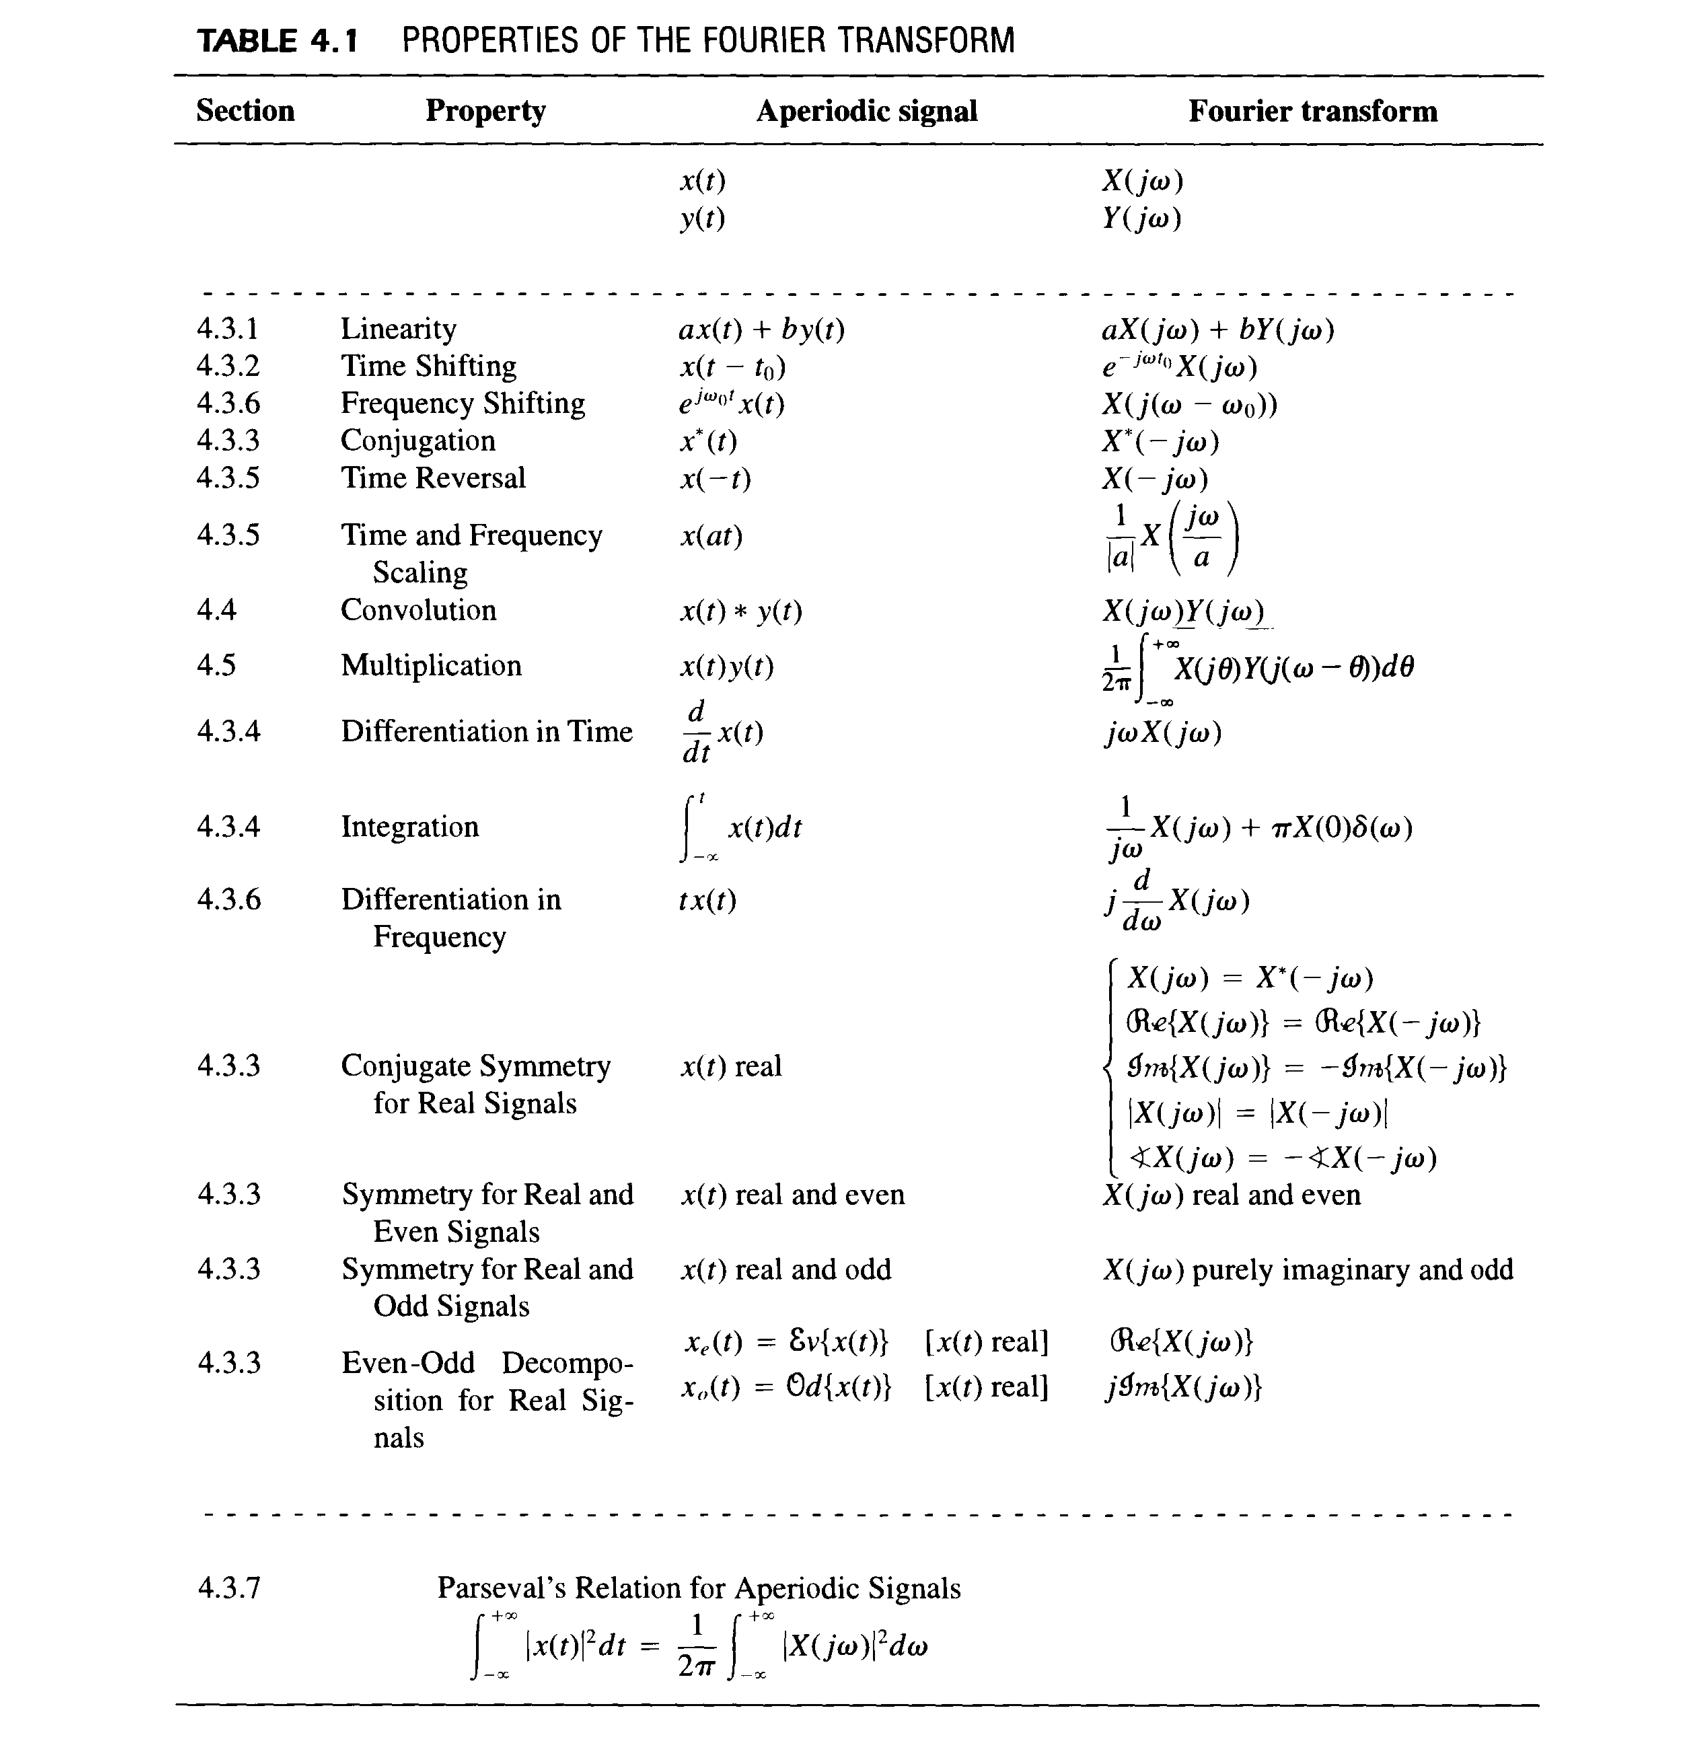
\includegraphics[width=0.8\linewidth]{img/image_2022-11-02-16-50-54.png}
	\caption{a pretty good table}
\end{figure}















































\end{document}
